\documentclass[twocolumn]{article}
\usepackage{movie15}
\usepackage{animate}
\usepackage{calc}
\usepackage{ifthen}
\usepackage[margin=0.5in]{geometry}
\usepackage{amsmath,amsthm,amsfonts,amssymb}
\usepackage{amsfonts}
\usepackage{color,overpic}
\usepackage{hyperref}
\usepackage{array} 
\usepackage{amstext}
\usepackage{enumitem}
\usepackage{graphicx}
\usepackage{caption}
\usepackage{natbib}
\usepackage{framed}
\usepackage{float}

\newenvironment{Figure}
  {\par\medskip\noindent\minipage{\linewidth}}
  {\endminipage\par\medskip}
  
\numberwithin{equation}{section}

\graphicspath{ {./Illustration/} }

% Turn off header and footer
\pagestyle{empty}

\setlist{leftmargin=0cm}
\setlist{noitemsep}

\title{Kalman-Filter}
\date{\vspace{-6ex}}

% -----------------------------------------------------------------------

\begin{document}
\maketitle


\section{Introduction}
	\subsection{Historical Development}
\begin{itemize}
	\item The filter is named after Hungarian Rudolf E. Kálmán, although Thorvald Nicolai Thiele and Peter Swerling developed a similar algorithm earlier. 
	\item Stanley F. Schmidt is credited for the first implementation of Kalman-filter to the problem of trajectory estimation for the Apollo program.
\end{itemize}
	
	\subsection{Overview}
Kalman filtering, (or linear quadratic estimation (LQE)), operates recursively on streams of noisy input data to produce a statistically optimal estimate of the underlying system state.

The algorithm works in a two-step process:
\begin{enumerate}
	\item \emph{Prediction step}: the Kalman filter produces estimates of the current state variables $\hat{\mathbf{x}}_{k|k-1}$, along with their uncertainties $\hat{\mathbf{P}}_{k|k-1}$.
	\item \emph{Update step}: Once the outcome of the next measurement ($\hat{\mathbf{y}}_k$) is observed, these estimates are updated ($\hat{\mathbf{x}}_{k|k}$ and $\hat{\mathbf{P}}_{k|k}$).
\end{enumerate}

\begin{figure}[H]
    \centering
    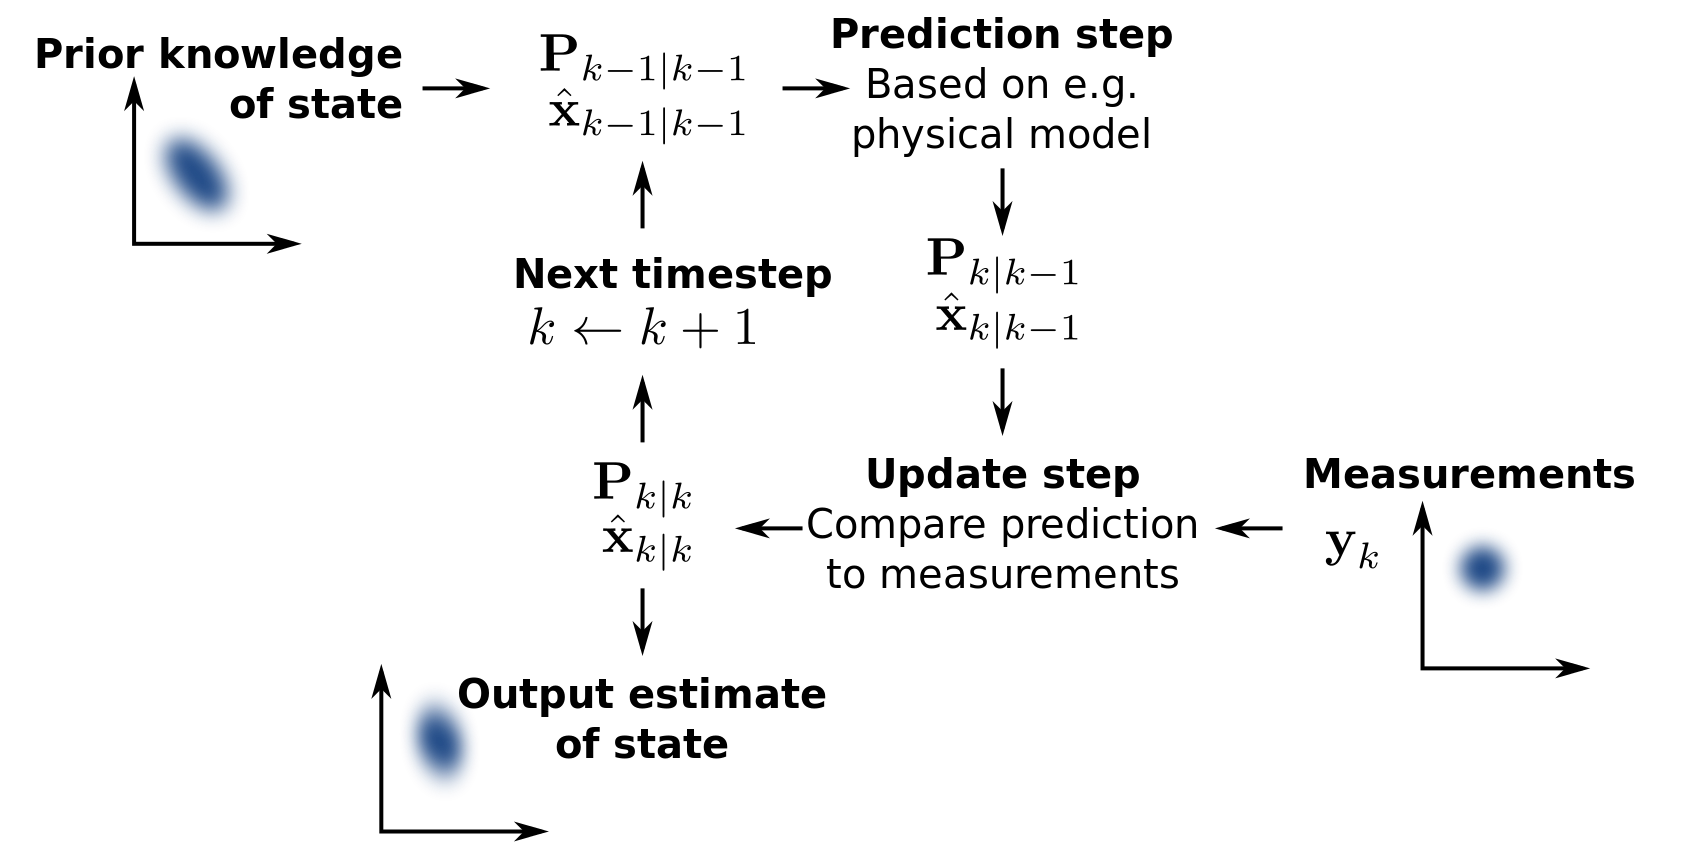
\includegraphics[width=.49\textwidth]{Basic_concept_of_Kalman_filtering.png}
\end{figure}


\newpage
\section{Kalman-Filter}	
	\subsection{Description}
The Kalman filter model assumes the true state to be based on linear dynamic systems discretized in the time domain:
 $$ \mathbf{x}_{k} = \mathbf{F}_{k} \mathbf{x}_{k-1} + \mathbf{B}_{k} \mathbf{u}_{k} + \mathbf{w}_{k}$$

where:
\begin{itemize}
	\item[-] $\mathbf{F}_{k}$ is the state transition model.
	\item[-] $\mathbf{B}_{k}$ is the control-input model.
	\item[-] $\mathbf{u}_{k}$ is the control vector.
	\item[-] $\mathbf{w}_{k}$ is the process noise of covariance $\mathbf{Q}_k$. $\mathbf{w}_{k} \sim \mathcal{N}(0, \mathbf{Q}_k)$ 
\end{itemize}

At time $k$, observation of $\mathbf{x}_k$ is mad according to
$$\mathbf{z}_k = \mathbf{H}_{k} \mathbf{x}_k + \mathbf{v}_k$$
where:
\begin{itemize}
	\item[-] $\mathbf{H}_{k}$ is the observation model
	\item[-] $\mathbf{v}_{k} \sim \mathcal{N}(0, \mathbf{R}_k)$ is the observation noise of covariance $\mathbf{R}_k$. 
\end{itemize}


\begin{enumerate}
	\item \emph{Prediction step}:
\end{enumerate}
\begin{tabular}{ p{.25\textwidth}p{.25\textwidth} }
A priori state estimate	& $\hat{\mathbf{x}}_{k\mid k-1} = \mathbf{F}_{k}\hat{\mathbf{x}}_{k-1\mid k-1} + \mathbf{B}_{k} \mathbf{u}_{k}$\\
A priori estimate cov. & $\mathbf{P}_{k\mid k-1} =  \mathbf{F}_{k} \mathbf{P}_{k-1\mid k-1} \mathbf{F}_{k}^{\text{T}} + \mathbf{Q}_{k}$ 
\end{tabular}
\begin{enumerate}[resume]
	\item \emph{Update step}: \newline
\end{enumerate}
\begin{tabular}{ p{.25\textwidth}p{.25\textwidth} }
Measurement residual	&
$\tilde{\mathbf{y}}_k = \mathbf{z}_k - \mathbf{H}_k\hat{\mathbf{x}}_{k\mid k-1}$\\
Residual covariance	&
$\mathbf{S}_k = \mathbf{H}_k \mathbf{P}_{k\mid k-1} \mathbf{H}_k^T + \mathbf{R}_k $\\
Optimal Kalman gain	&
$\mathbf{K}_k = \mathbf{P}_{k\mid k-1}\mathbf{H}_k^T \mathbf{S}_k^{-1}$\\
A posteriori state estimate	&
$\hat{\mathbf{x}}_{k\mid k} = \hat{\mathbf{x}}_{k\mid k-1} + \mathbf{K}_k\tilde{\mathbf{y}}_k$\\
A posteriori estimate cov.	&
$\mathbf{P}_{k|k} = (I - \mathbf{K}_k \mathbf{H}_k) \mathbf{P}_{k|k-1}$\\
\end{tabular}

\begin{figure}[H]
    \centering
    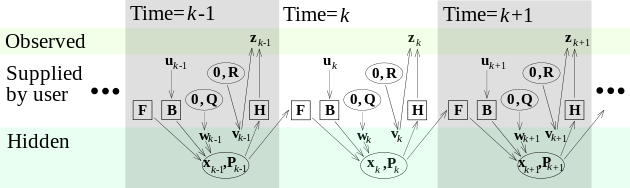
\includegraphics[width=.49\textwidth]{Kalman_filter_model_2.png}
\end{figure}



	\subsection{Practical Application}
\begin{itemize}
	\item Unknown stochastic signals as input can seriously degrade the filter performance. Robust Control is then used.
	\item One major practical challenge is finding the covariance of the noise ($\mathbf{Q}_k$ and $\mathbf{R}_k$). One of the more promising approaches is the Autocovariance Least-Squares (ALS) technique that uses the time-lagged autocovariances of routine operating data.
\end{itemize}





\section{Extension}
	\subsection{Recursive Bayesian Estimation}
Recursive Bayesian estimation, also known as a Bayes filter, is a general probabilistic approach for estimating an unknown probability density function recursively over time using incoming measurements and a mathematical process model.



\begin{figure}[H]
    \centering
    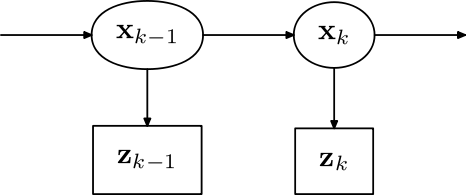
\includegraphics[width=.49\textwidth]{466px-HMM_Kalman_Filter_Derivation.png}
\end{figure}








\bibliographystyle{apalike}
\bibliography{citations}	
	

\end{document}